\documentclass[11pt]{article}
\usepackage{amsmath, amssymb, amsthm}
\usepackage[retainorgcmds]{IEEEtrantools}

\usepackage[pdftex]{graphicx}
\usepackage{tikz}
\usetikzlibrary{intersections}

\usepackage{fancyhdr}

%Listings stuff
\usepackage{listings}
\usepackage{lstautogobble}
\usepackage{color}

\definecolor{gray}{rgb}{0.5,0.5,0.5}
\lstset{
basicstyle={\small\ttfamily},
tabsize=3,
numbers=left,
numbersep=5pt,
numberstyle=\tiny\color{gray},
stepnumber=2,
breaklines=true,
boxpos=t
}

%Format stuff
\pagestyle{fancy}
\headheight 35pt

%Header info
\chead{\Large \textbf{Prim's Algorithm}}
\lhead{}
\rhead{}

\begin{document}
\section{Example}
	\begin{center}
	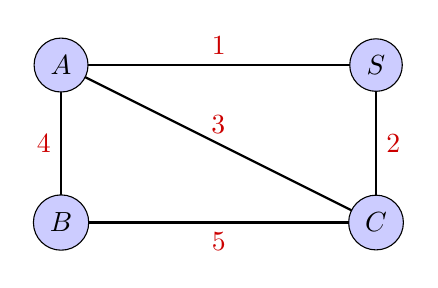
\begin{tikzpicture}
		[scale=1,line cap=round,
		%Styles
		axes/.style=,
		important line/.style={very thick},
		information text/.style={rounded corners,fill=red!10,inner sep=1ex},
		dot/.style={circle,inner sep=1pt,fill,label={#1},name=#1},
		node/.style={circle,fill=blue!20,draw}				
		]
		
		%Colors
		\colorlet{anglecolor}{green!50!black}	%angle arcs/lines
		
		%The graphic
		\node[node] (S) at (4, 2) {$S$};
		\node[node] (A) at (0, 2) {$A$};
		\node[node] (B) at (0, 0) {$B$};
		\node[node] (C) at (4, 0) {$C$};
		
		\path[thick]
			(A) edge node[left,red!80!black] {$4$} (B)
				edge node[above,red!80!black] {$3$} (C)
				edge node[above,red!80!black] {$1$} (S)
			(S) edge node[right,red!80!black] {$2$} (C)
			(B) edge node[below,red!80!black] {$5$} (C);
	\end{tikzpicture}
	\end{center}
	
	Prim's algorithm begins with picking an arbitrary source vertex, in this example labeled $S$. Until the tree contains all of the vertices, expand the MST by choosing the cheapest edge that adds a vertex to the subgraph.
	\begin{center}
	\begin{tabular}{ccc}
		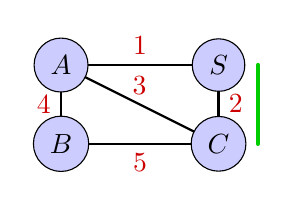
\begin{tikzpicture}
			[scale=.5,line cap=round,
			%Styles
			axes/.style=,
			important line/.style={very thick},
			information text/.style={rounded corners,fill=red!10,inner sep=1ex},
			dot/.style={circle,inner sep=1pt,fill,label={#1},name=#1},
			node/.style={circle,fill=blue!20,draw}				
			]
			
			%Colors
			\colorlet{anglecolor}{green!50!black}	%angle arcs/lines
			
			%The graphic
			\node[node] (S) at (4, 2) {$S$};
			\node[node] (A) at (0, 2) {$A$};
			\node[node] (B) at (0, 0) {$B$};
			\node[node] (C) at (4, 0) {$C$};
			
			\path[thick]
				(A) edge node[left,red!80!black] {$4$} (B)
					edge node[above,red!80!black] {$3$} (C)
					edge node[above,red!80!black] {$1$} (S)
				(S) edge node[right,red!80!black] {$2$} (C)
				(B) edge node[below,red!80!black] {$5$} (C);
				
			\draw[green!80!black, ultra thick] (C) +(1, 0) -- +(1, 2);
		\end{tikzpicture}
		&
		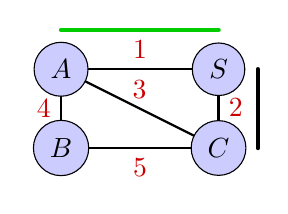
\begin{tikzpicture}
			[scale=.5,line cap=round,
			%Styles
			axes/.style=,
			important line/.style={very thick},
			information text/.style={rounded corners,fill=red!10,inner sep=1ex},
			dot/.style={circle,inner sep=1pt,fill,label={#1},name=#1},
			node/.style={circle,fill=blue!20,draw}				
			]
			
			%Colors
			\colorlet{anglecolor}{green!50!black}	%angle arcs/lines
			
			%The graphic
			\node[node] (S) at (4, 2) {$S$};
			\node[node] (A) at (0, 2) {$A$};
			\node[node] (B) at (0, 0) {$B$};
			\node[node] (C) at (4, 0) {$C$};
			
			\path[thick]
				(A) edge node[left,red!80!black] {$4$} (B)
					edge node[above,red!80!black] {$3$} (C)
					edge node[above,red!80!black] {$1$} (S)
				(S) edge node[right,red!80!black] {$2$} (C)
				(B) edge node[below,red!80!black] {$5$} (C);
				
			\draw[black, ultra thick] (C) +(1, 0) -- +(1, 2);
			\draw[green!80!black, ultra thick] (S) + (0, 1) -- +(-4, 1);
		\end{tikzpicture}
		&
		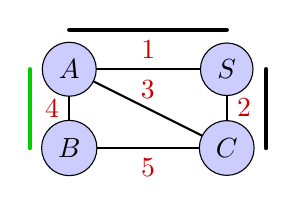
\begin{tikzpicture}
			[scale=.5,line cap=round,
			%Styles
			axes/.style=,
			important line/.style={very thick},
			information text/.style={rounded corners,fill=red!10,inner sep=1ex},
			dot/.style={circle,inner sep=1pt,fill,label={#1},name=#1},
			node/.style={circle,fill=blue!20,draw}				
			]
			
			%Colors
			\colorlet{anglecolor}{green!50!black}	%angle arcs/lines
			
			%The graphic
			\node[node] (S) at (4, 2) {$S$};
			\node[node] (A) at (0, 2) {$A$};
			\node[node] (B) at (0, 0) {$B$};
			\node[node] (C) at (4, 0) {$C$};
			
			\path[thick]
				(A) edge node[left,red!80!black] {$4$} (B)
					edge node[above,red!80!black] {$3$} (C)
					edge node[above,red!80!black] {$1$} (S)
				(S) edge node[right,red!80!black] {$2$} (C)
				(B) edge node[below,red!80!black] {$5$} (C);
				
			\draw[black, ultra thick] (C) +(1, 0) -- +(1, 2);
			\draw[black, ultra thick] (S) + (0, 1) -- +(-4, 1);
			\draw[green!80!black, ultra thick] (A) +(-1, 0) -- +(-1, -2);
		\end{tikzpicture}
	\end{tabular}
	\end{center}
	
	In the above example, the final result yields $|MST| = 7$.
	
\section{Algorithm}
	\begin{lstlisting}[autogobble=true]
		def Prim(G=(V,E), S):
			X = {S}, T = null
			while X != V:
				e = (u, v)	#Cheapest edge | u in X and v not in X
				T += e
				X += v
	\end{lstlisting}
	
\section{Correctness}
	Split the proof of correctness into two parts: first that the algorithm correctly computes a spanning tree $T^*$, then that $T^*$ is an MST.
	
	\subsection{Spanning Proof}
		Given that a cut of $G$ is a partition of $V$ into two non-empty groups, we can define the following three properties:
		\begin{enumerate}
			\item \textbf{Empty cut lemma:} $G$ is not connected if and only if there exists a cut with no crossing edges.
			\item \textbf{Double-crossing lemma:} if a cycle $C\subset E$ crosses the cut, then it must cross back as well.
			\item \textbf{Lonely-cut corollary:} If $e$ is the only edge crossing a cut, it is not in a cycle.
		\end{enumerate}
		
		Prim's algorithm maintains the invariant that $T$ always spans $X$, for obvious reasons. The algorithm also can never get ``stuck'' (i.e., no more edges to add) in a state such that $X \neq V$, because otherwise the cut $(X, V-X)$ must be empty, and by the empty-cut lemma $G$ would be disconnected. Therefore, the algorithm finishes when $X = V$, and because of the invariant, $T$ spans $V$.
		
		The spanning tree computed by the algorithm also cannot cycle. Consider a snapshot of the algorithm at any iteration, which has in a sense partitioned the graph into the cut $(X, V-X)$. Obviously, no edge in $T$ crosses this cut because they all connect vertices in $X$. On the next iteration, after adding an edge $e$, it must be the only edge crossing the cut, and by the lonely-cut corollary, it cannot be part of a cycle.
		
		Putting together those two conditions, that $T$ spans $V$ and does not contain any cycles, we prove that Prim's algorithm outputs a spanning tree.
		
	\subsection{Minimum Proof}
		To prove that Prim's algorithm outputs a minimum spanning tree and not just any spanning tree, consider the \textbf{cut property}.
		
		\subparagraph{Cut Property} Consider an edge $e\in E$. Suppose there exists a cut $(A, B)$ of $G$ such that $e$ is the cheapest crossing edge. Then $e$ must belong to the MST of $G$.
		
		Now remember that in each iteration of the algorithm the graph is partitioned into a cut $(X, V-X)$. By the definition of the algorithm, it chooses the cheapest edge that crosses this cut. Therefore, by the cut property, Prim's algorithm always picks edges in the MST.
%	\begin{center}
%	\begin{tikzpicture}
%		[scale=3,line cap=round,
%		%Styles
%		axes/.style=,
%		important line/.style={very thick},
%		information text/.style={rounded corners,fill=red!10,inner sep=1ex},
%		dot/.style={circle,inner sep=1pt,fill,label={#1},name=#1}			
%		]
%		
%		%Colors
%		\colorlet{anglecolor}{green!50!black}	%angle arcs/lines
%		
%		%The graphic
%	\end{tikzpicture}
%	\end{center}

%	\begin{figure}[htb]
%		\centering
%		\includegraphics[width=0.8\textwidth]{filename.eps}
%		\caption{Caption.}
%		\label{fig:figure}
%	\end{figure}

%		\def\enotesize{\normalsize}
%		\theendnotes
\end{document}